\documentclass[12pt,letterpaper]{article}
\usepackage{amsmath,amsthm,amsfonts,amssymb,amscd}
\usepackage{fullpage}
\usepackage{lastpage}
\usepackage{enumerate}
\usepackage{fancyhdr}
\usepackage{mathrsfs}
\usepackage{xcolor}
\usepackage{dsfont}
\usepackage{graphicx}
\usepackage[framed]{mcode}
\usepackage[margin=3cm]{geometry}
\setlength{\parindent}{0.0in}
\setlength{\parskip}{0.05in}

% Edit these as appropriate
\newcommand\course{CIS 581}
\newcommand\semester{Fall 2014}     % <-- current semester
\newcommand\yourname{Michael O'Meara, Mike Woods} % <-- your name
\newcommand\hwdate{Due: December 20, 2014}           % <-- HW due date

\newenvironment{answer}[1]{
  \subsubsection*{Our #1}
}


\pagestyle{fancyplain}
\headheight 25pt

\lhead{\\\course\ --- \semester}
\chead{\textbf{\Large Face Replacement \hwnum}}
\rhead{\hwdate}

\headsep 5pt

\begin{document}

\text{\yourname}

\begin{answer}{approach}

\begin{enumerate}

\item Initially we used the code published by Zhu and Ramanan based on a paper called "Face Detection, Pose Estimation and Landmark Localization in the Wild" to perform landmark detection on the input or reference faces.  This approach uses a deformable template to find key features in the face.
\begin{enumerate}

\item We used this to find points for the eyes, nose, and mouth.


% So far, one of most challenging sub-problems we've encountered has to do with obtaining a clear outline of the face, specifically the jawline. The code by Zhu and Ramanan performs this task fairly well in most test images we've tried.

\item Using these points, we dilate the centers of those points into circles.  
\item Then, with those circles, we calculate a mask of both the reference images and the target images. 

\item NOTE: since the points in the template remain roughly in the same positions on each face, this makes our approach fairly stable.

% We will later use both to extract the actual face from the input image and create a hole in the target image for adding the convex hull of the reference image. 

\end{enumerate}

% \item After trying many different approaches involving localized feature detection in order to match points with no real success, we finally found code published by Serge Belongie, Jitendra Malik and Jan Puzicha on matching point features using Shape Context.  Their code uses Hungarian Bipartite graph matching and gave us almost perfect point correspondence between the reference and target image as can be seen in our results on the next page.

%\item Additionally, we also construct a bounding box/region of interest based on the initial set of detected facial points which we use to perform localized feature detection, identifying the nose, eyes, and mouth. The location of the nose is also used to perform left eye/right eye disambiguation and remove false positives. 

%\item Our next task is to detect the best corners within the local feature bounding boxes (most likely on the eyes and mouth) of the source and target images in order to prune dissimilar correspondence points in both the target and source images. 
\item We thought we'd need to use Thin-Plate Spline warping but, that turned out not to be necessary.

\item Instead, we do an affine transform to adjust the angle of our face to match the target face(s).

\item Lastly, we decided to do three different levels of blending to match the surrounding target face.

\end{enumerate}

\end{answer}


\begin{answer}{results}

\begin{figure}[!ht]
        \caption{Shape context point matching}
\center
%        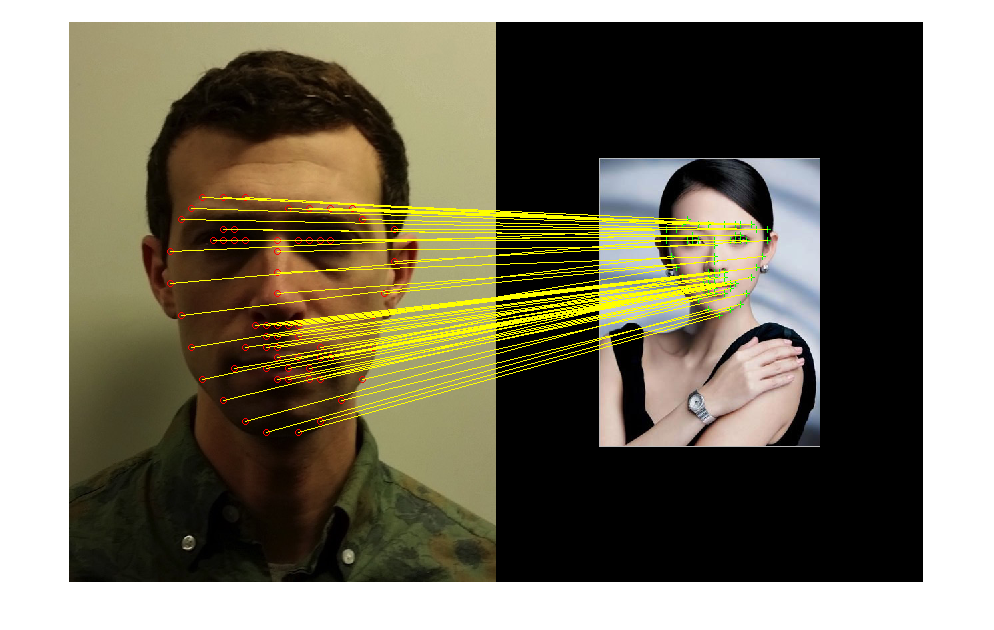
\includegraphics[scale=0.25]{match_1}
        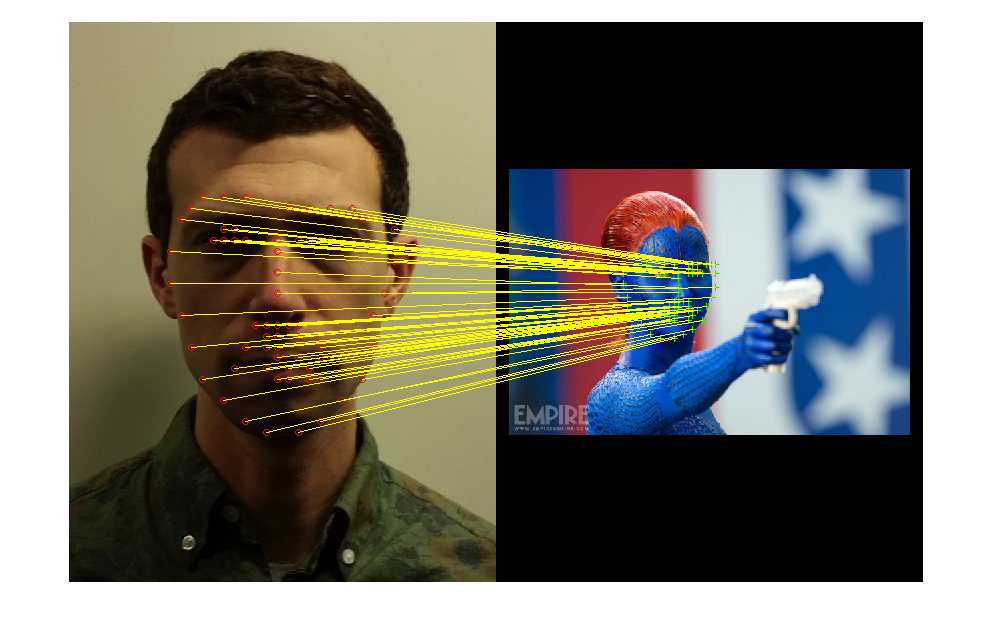
\includegraphics[scale=0.3]{match_2}
        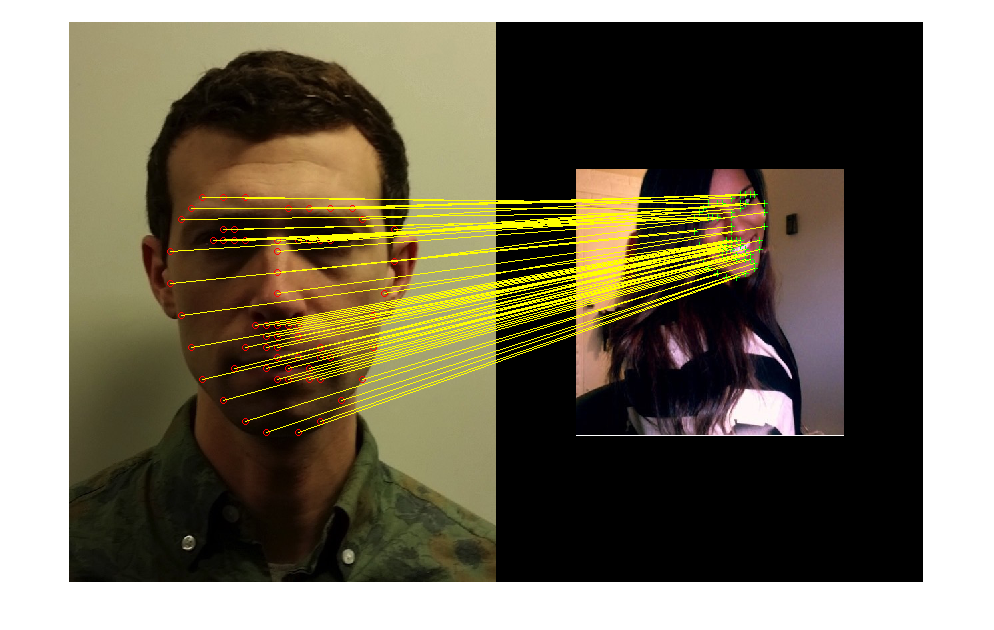
\includegraphics[scale=0.3]{match_3}
        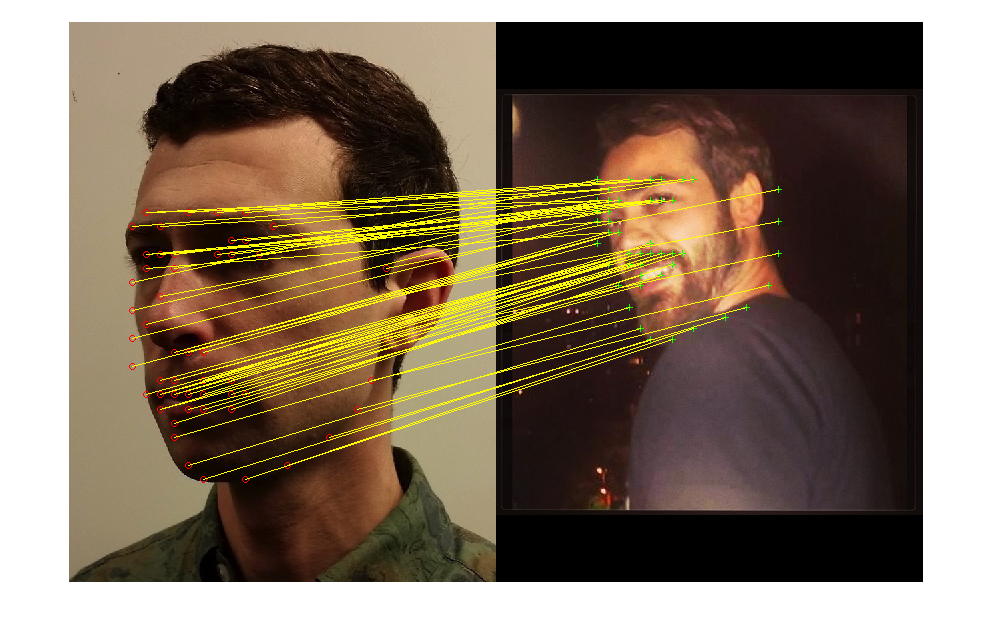
\includegraphics[scale=0.3]{match_4}
\end{figure}


\end{answer}


\end{document}


